\chapter{The role of vertical structure in QBO teleconnections}
\label{cha:deepQBO}

\section{Introduction}
\label{sec:deepQBO-introduction}
The QBO is typically defined by the equatorial ZMZW at a single level in the mid-stratosphere. The 50 hPa level is usually used for NH observational studies \citep{Baldwin2001, Baldwin98} but some studies have also noted the importance of characterising the vertical structure of the QBO \citep{Fraedrih1993, Wallace1993,  Baldwin98,  Dunkerton2017, Gray2018, andrewsObserved2019}. In an observational-based study \cite{Gray2018} find an enhanced association between the QBO and polar vortex when a metric incorporating the vertical coherence of equatorial winds via empirical orthogonal functions is utilised \citep{verena2016a}. In a model-based study \cite{Andrews2019} introduce a similar but simpler methodology by defining the QBO as the average ZMZW between two vertical levels, which preferentially selects time intervals that display a vertically coherent QBO phase between the specified levels. The same study reports enhanced responses to the QBO from the NAO and Arctic Oscillation (AO) when such vertically integrated metrics are used to define QBO phase compared to a single level definition. While these studies highlight statistical associations between vertical QBO metrics and the vortex, the importance of vertical coherence in HT strength has not been tested explicitly. Furthermore, influence mechanisms are not well understood. 


\section{Model Configuration}

To explicitly test the effect of QBO vertical coherence on teleconnections we utilise a set of custom designed simulations which utilises a modified version of the UKESM GCM analysed in chapters 3 and 4. As with the pi-control simulation examined so far, the model component for the atmosphere is GA7.1, GHG concentrations are set to 1850 levels (see section \ref{sec:model_config}) and volcanic eruptions are absent (however a constant background volcanic aerosol level is imposed). The primary difference between the pi-control and the configuration utilised here is the experiments run with no coupled Ocean component. Instead, SSTs are prescribed using a seasonally invariant climatological field obtained from an interval of the the pi-control (year numbers 96-126). Sea Ice extents are also prescribed to climatological values using the same interval of the pi-control and full documentation for this type of timeslice experiment is provided in \cite{oconnorAssessment2021}. All simulations are initialised using conditions from the start of the 30 year interval of the pi-control used to calculate SST and SI climatologies (year number 96). We choose to impose SST and sea ice conditions in our experiments as this removes contributions to atmospheric circulation from interannual to decadal surface modes of variability such as ENSO and the AL. This in turn isolates the effect of the QBO further as any differences in QBO-vortex and QBO-surface interactions across the simulations are not due to coupling with SSTs and other surface boundary conditions.  %Analysis chapters 4 and 5 showed that this year does not lie in an interval in which the QBO or the vortex exhibits significant multi-decadal oscillations. As a result, the initial conditions for the simulation are less likely samples the QBO and vortex in a randomly chosen state.

\section*{Nudging}
In order to impose the vertical structure of the QBO in our sensitivity experiments we employ a method to constrain atmospheric conditions in a GCM simulation known as nudging. In this method, an atmospheric quantity, $Y$, is constrained via Newtonian-relaxation which pushes the model state for $Y$ towards some imposed value at each model timestep such that

\begin{equation} \label{eq:nudging}
\Delta Y = G \Delta t (Y_{imposed} - Y_{model}), 
\end{equation}

where $Y_{imposed}$ is the state of $Y$ from the imposed field, $Y_{model}$ is the value of $Y$ the model has evolved to since the last timestep (when it was last nudged), $\Delta Y$ is the change in $Y$ applied by the nudging scheme and $G$ is the relaxation parameter. $G$ is a measure of the strength of the relaxation towards $Y_{imposed}$ at each timestep and can also be expressed as $G = \frac{1}{\tau}$ where $\tau$ is known as the relaxation timescale. When choosing the relaxation timescale, a balance is required between constraining the model sufficiently to the imposed state (I.E. a short enough $\tau$ such that the model $Y$ avoids evolving freely) and avoiding the introduction of large gradients (a large enough $\tau$ to avoid model instability). The MetOffice Unified model, of which the model configurations presented here are a part, typically uses a relaxation timescale of 6 hours at all vertical levels. This has been shown to produce good quality nudging results in a range of studies employing such a method despite the different radiative timescales present across atmospheric levels (Brown et al. 2020). In our experiments we to nudge the zonal wind, $U$, towards an idealised version of the QBO wind fields expressed as 

\begin{equation} \label{eq:imposed_U}
U_{qbo}(t, z) = F(z) sin(\frac{2\pi (t + zs)}{period}),
\end{equation}

Where $s$ is a parameter which sets the rate of phase shift with descending height. We set $s$ to xxxx and the For the deep QBO experiment (that which displays a high degree of vertical coherence) and xxx for the shallow QBO to ensure a large phase shift with height (and therefore less vertical coherence). We choose the period of the QBO in both experiments to be xxx months for consistency with the QBO period exhibited in the UKESM pi-control. $F(z)$ is a momentum forcing vertical profile (seen in figure xxx) applied to reproduce the variation in magnitude of the QBO with height. Following the methodology of Pascoe et al., we use an $F(z)$ which takes the form of a Weibull function given by

\begin{equation} \label{eq:vertical_profile}
F(z) = R_D \frac{1}{\gamma \beta^\alpha}  Z_D^{\alpha-1}  e^{-Z_D/\beta},
\end{equation}

where the parameters are set to $\alpha = 3.5, \beta = 0.27, \gamma = 3.2335, R_D = 40.0 ms^{-1}, Z_{D} = (z - 15)/20$. The idealised time-height QBO profiles generated for both experiments are shown in figure xxxxa, they highlight the differences between idealised QBOs: The deep QBO winds exhibits the same sign of wind throughout the middle atmosphere for the majority of the series while the shallow QBO show different phases between the upper and middle stratosphere. In both experiments we apply the relaxation in equation \ref{eq:nudging} towards the corresponding QBO winds over the set of atmospheric levels approximately corresponding to the pressure level range xx-xxhPa and the latitudinal range xx-xx. The relaxation is applied at all longitudes. At the boundary between of these ranges we apply a tapered version of the relaxation with a value of that parameter $G$ that decreases linearly with increased distance from the relaxation region. This tapering is applied on the 2 atmospheric levels at the bottom and top of the vertical region and 5$^\circ$ either side of the latitudinal region. This tapering is applied to avoid introducing large vertical and latitudinal gradients in zonal wind and prevent potential model instability. 

\begin{figure}[h!]
\begin{center}
\noindent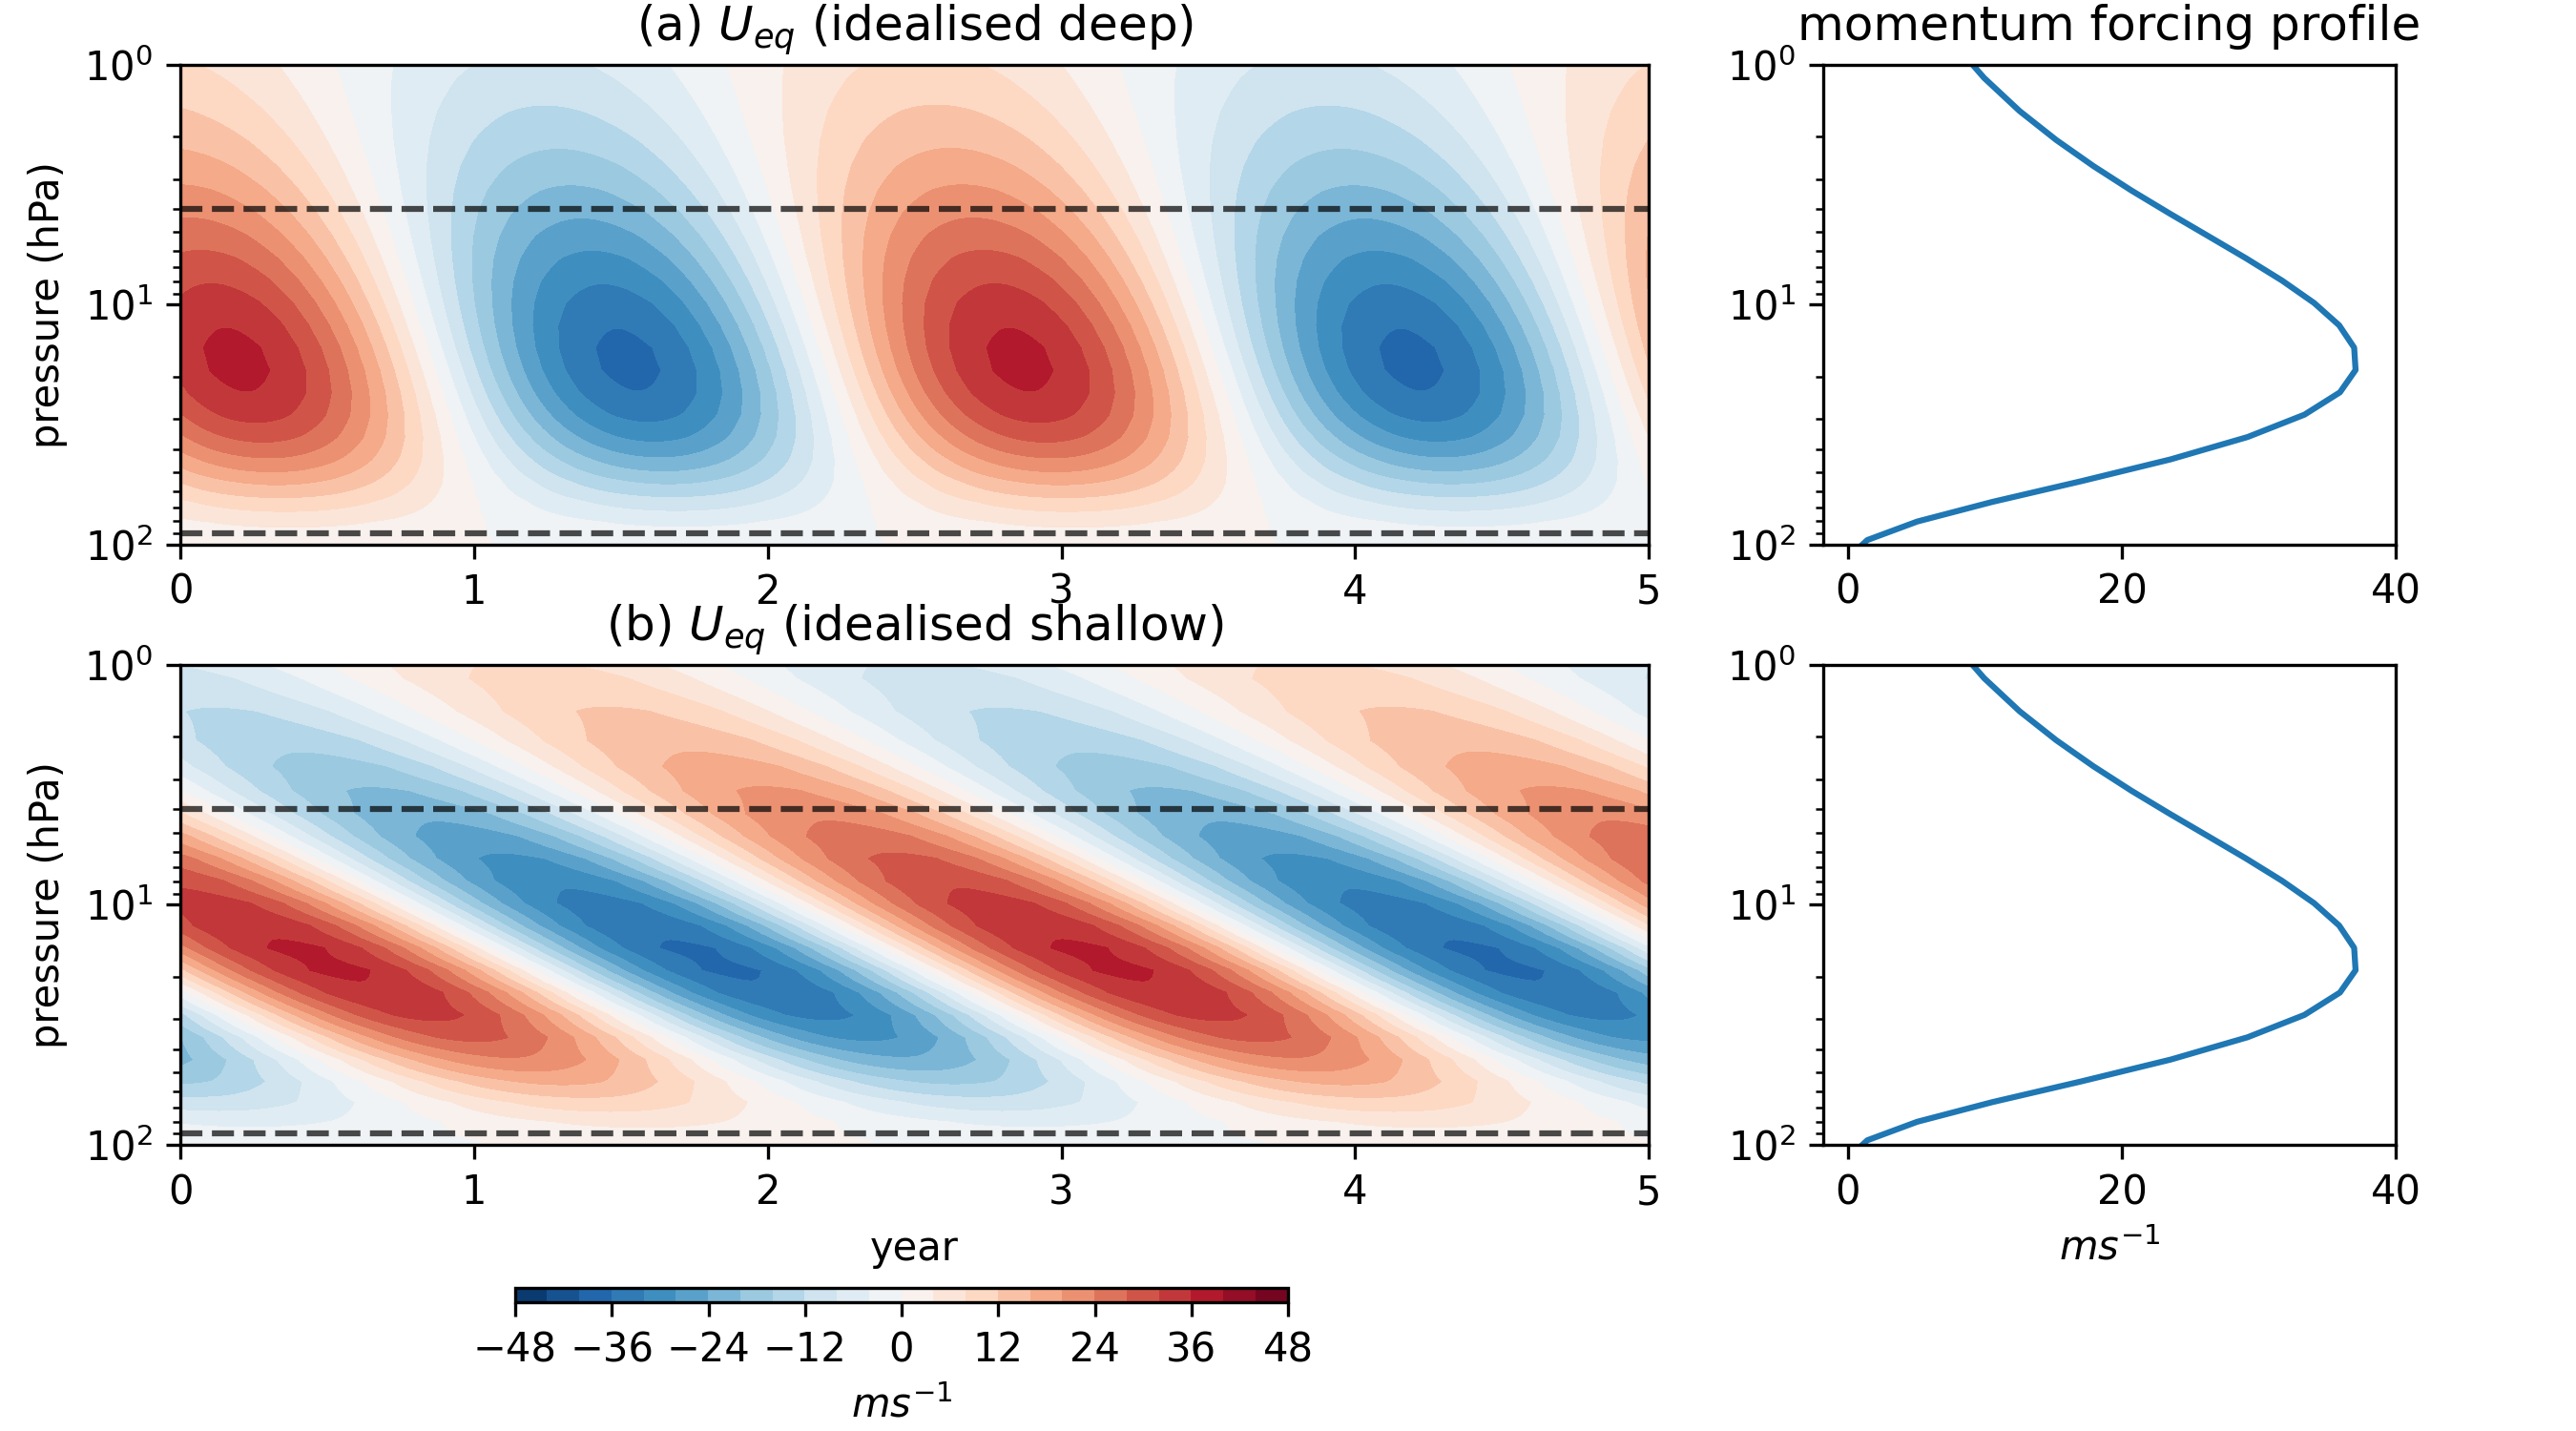
\includegraphics[width = \linewidth]{Figures/Figures-deepQBO/Idealised_QBO_features.png}
\caption[Idealised QBO winds used for nudging experiments]{Sample time-series of idealised equatorial ZMZW and associated momentum forcing profile for the deep (\textbf{a} and \text{b} respectively) and shallow (\textbf{c} and \textbf{d} respectively) QBO experiments. Horizontal dashed lines on (a) and (c) denote the xxhPa and 90hPa pressure levels between which we implement nudging towards the idealised wind in each experiment.}
\label{fig:Idealised_QBO_samples}
\end{center}
\end{figure}


\section{Results}
\subsection{QBO Characteristics}
We first analyse the equatorial winds in each experiment and verify if the implementation of nudging has resulted in realistic ZMZW profiles. Figure \ref{experiment_QBO_samples} shows the equatorial winds that results from implementing QBO nudging between the xxhPa and xxhPa levels. These winds reflect the key features of the idealised winds (figure \ref{fig:Idealised_QBO_samples}a and c) - the deep experiment exhibits vertical coherence in the middle stratosphere while the shallow simulation shows opposite phases of the QBO in the upper and lower stratosphere. This indicates that the selection of nudging timescale, $\tau$ = 6 hours, is suitable to fix the state of the QBO in each experiment. 

- notable SAO anomalies

- show winter climatology of each experiment which reflects the SAO anomalies. This could give an indication towards the 

\begin{figure}[h!]
\begin{center}
\noindent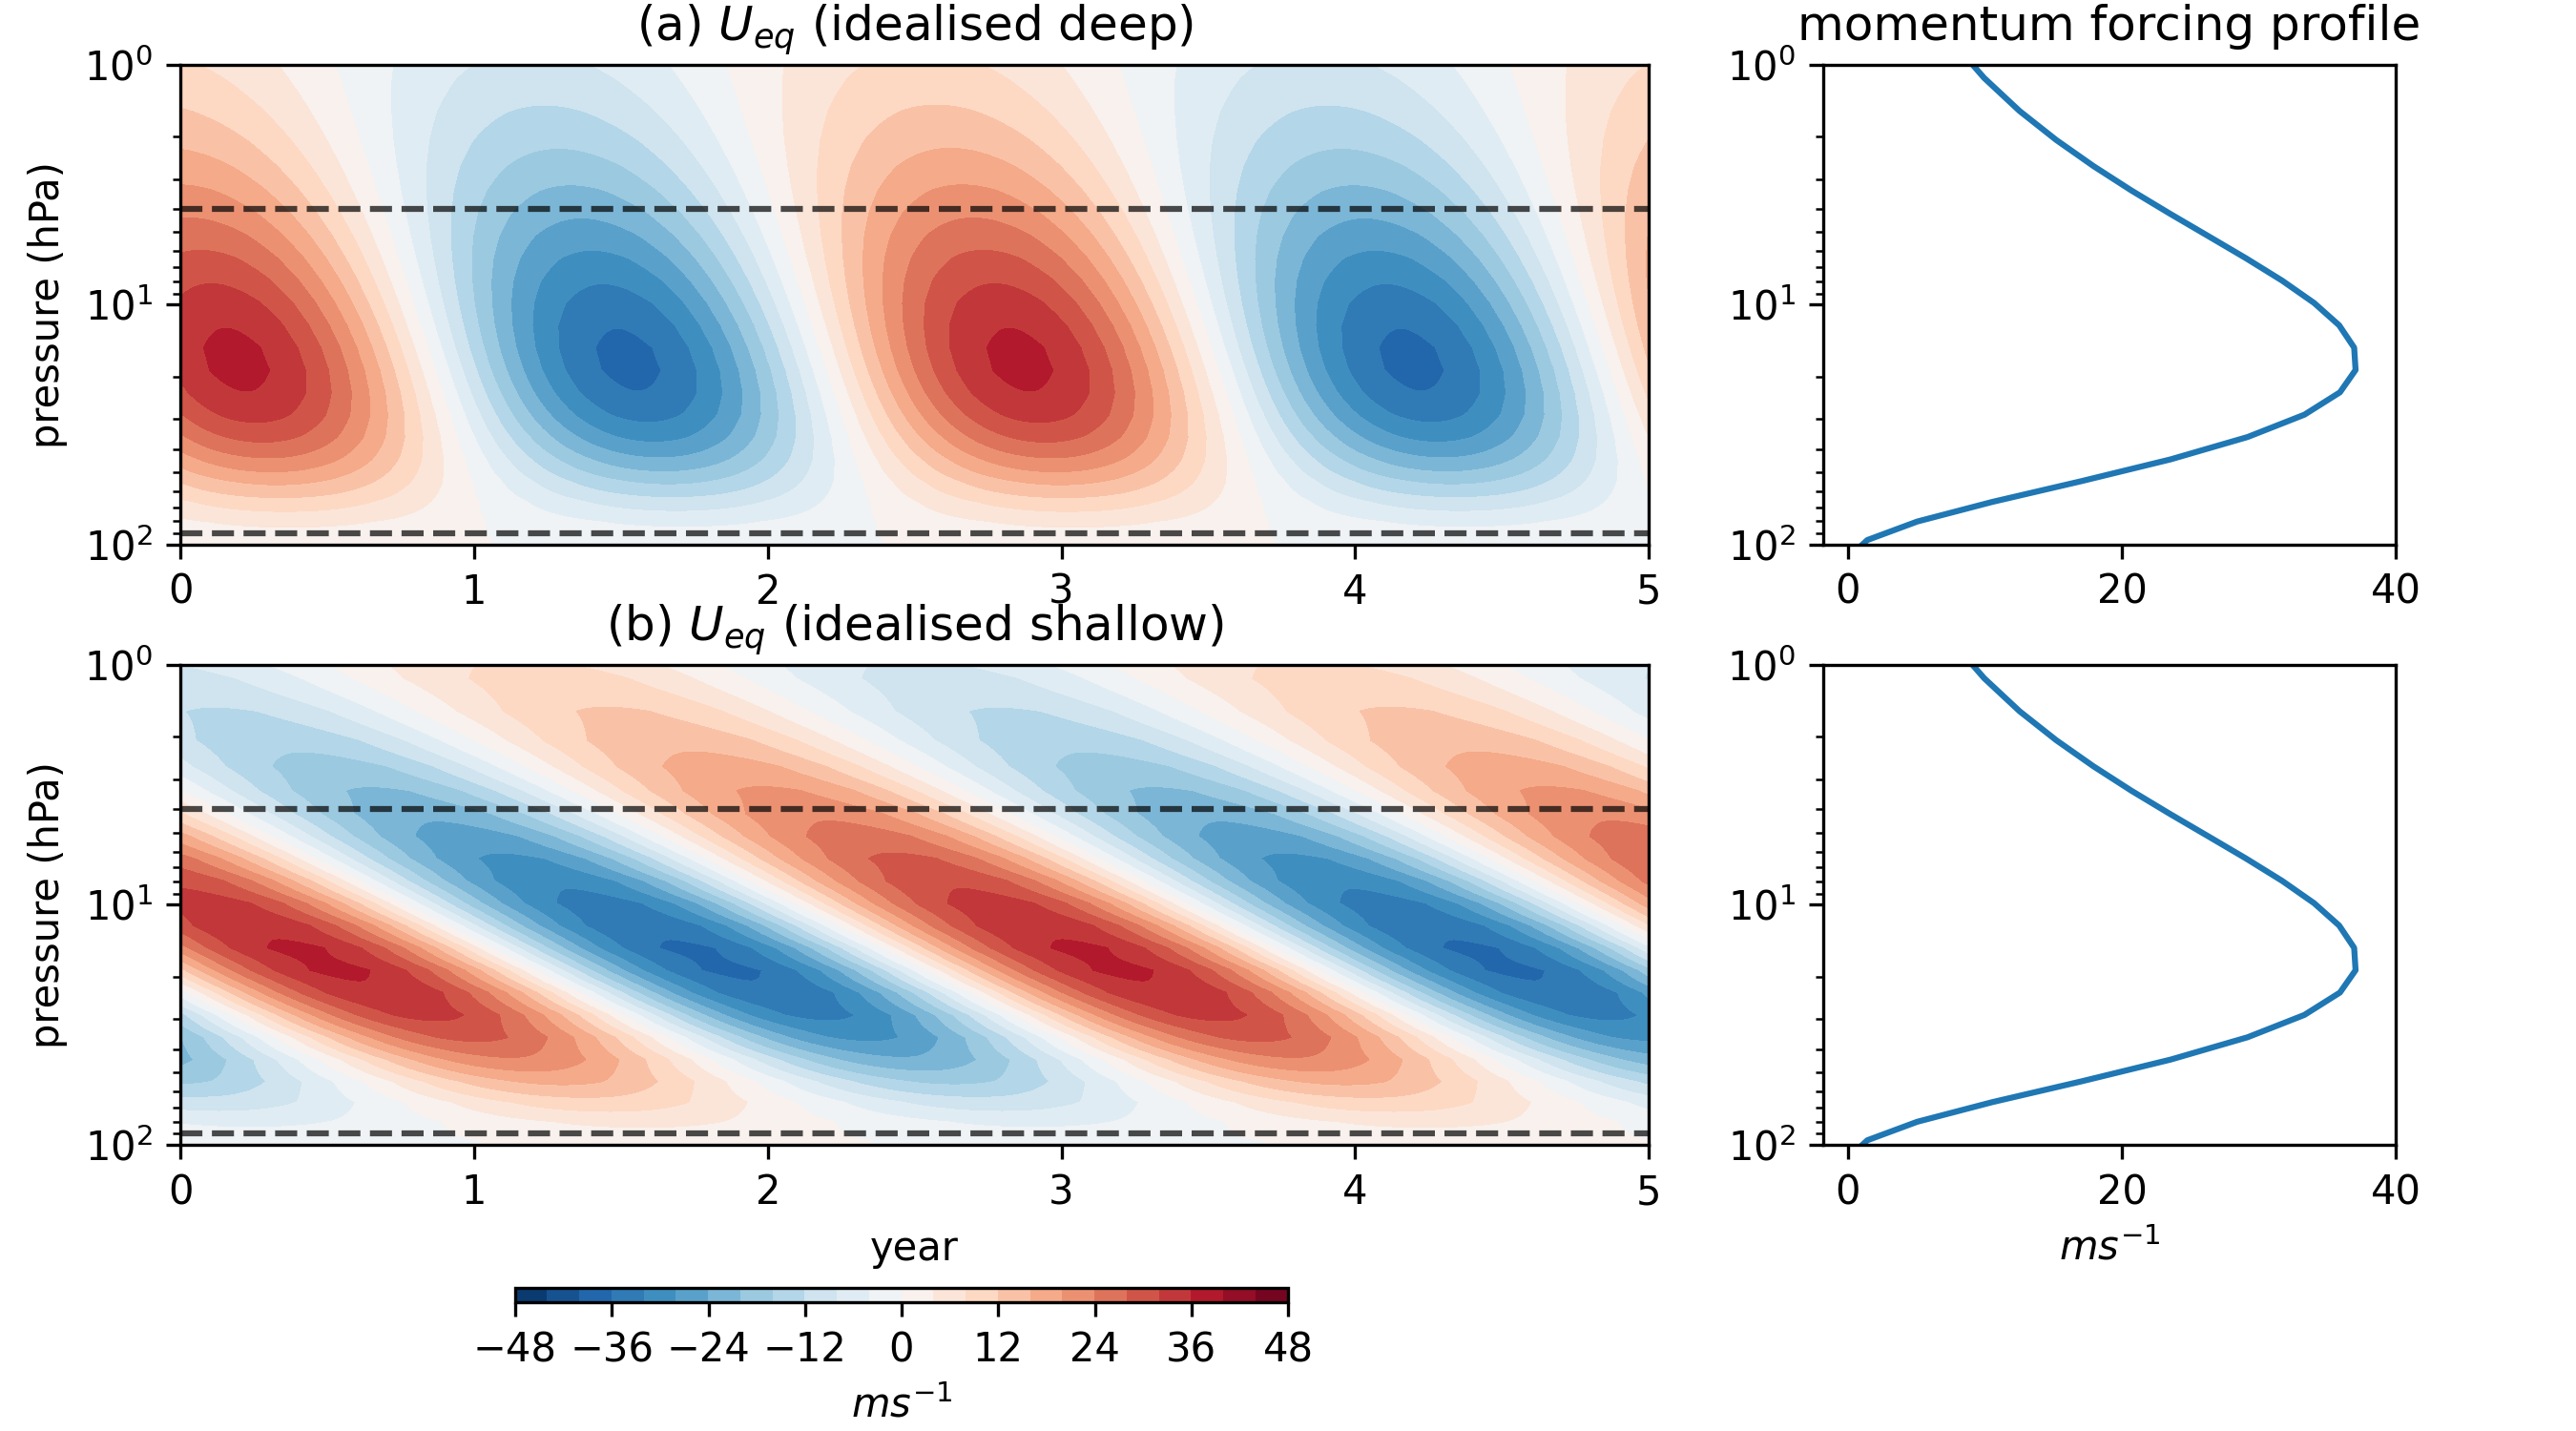
\includegraphics[width = \linewidth]{Figures/Figures-deepQBO/Idealised_QBO_features.png}
\caption[Idealised QBO winds used for nudging experiments]{Sample time-series of idealised equatorial ZMZW and associated momentum forcing profile for the deep (\textbf{a} and \text{b} respectively) and shallow (\textbf{c} and \textbf{d} respectively) QBO experiments. Horizontal dashed lines on (a) and (c) denote the xxhPa and 90hPa pressure levels between which we implement nudging towards the idealised wind in each experiment.}
\label{fig:Idealised_QBO_samples}
\end{center}
\end{figure}

We need to show first that the nudging we have implemented has resulted in realistic winds in the model. We don't want the idealised nudging to have 'messed up' other regions e.g. the SAO. We can use ERA-Interim composites to do this.

Fig1 - Nudged equatorial winds in each experiment as well as possible ERA-Interim or the pi-clim control for UKESM. Demonstrate that the nudging scheme has been effective in fixing the winds over the correct pressure level range. possibly include some height-period Fourier spectra for each QBO. 

Fig2 - a possible composite plot showing how the deep QBO manifests in the remainder of the atmosphere in ERA-Interim compared to that in each experiments. Need some argument showing a) that the deep QBO induces anomalies in the SAO region and b) that the deep QBO experiment show a similar SAO anomaly. 


\subsection{QBO teleconnections}



